\documentclass[10pt,twocolumn,letterpaper]{article}

%%%%%%%%% PAPER TYPE - same setting as the preliminary report
\usepackage[review]{cvpr}      % REVIEW version (as used in PPR16)
%\usepackage{cvpr}             % CAMERA-READY version (shows author names)

\usepackage{graphicx}
\usepackage{amsmath}
\usepackage{amssymb}
\usepackage{booktabs}
\usepackage{xcolor}

\usepackage[pagebackref,breaklinks,colorlinks]{hyperref}
\usepackage{cleveref}
\usepackage{etoolbox}
% Anything shown in red and in [square brackets] still has to be filled in.
\newcommand{\fillme}[1]{\textcolor{red}{[#1]}}

%%%%%%%%% PAPER ID
\def\cvprPaperID{PPR16}
\def\confName{CVPR}
\def\confYear{2023}

\begin{document}

%%%%%%%%% TITLE
\title{QPSK Midterm Report: FPGA-Oriented QPSK Modulator and Demodulator with Simulated AWGN Channel}

\author{Darsh Gajare, Parth Achat, Nishid Khandagre and Aditya Mali\\
Electrical Engineering\\
Indian Institute of Technology Hyderabad}
\maketitle

%%%%%%%%% ABSTRACT
\begin{abstract}
This report presents the mid-term progress of an FPGA-oriented Quadrature Phase Shift Keying (QPSK) modem for the EE2000 Signal Processing project. The system includes an NCO-based transmitter, a digitally modelled noisy channel, and a coherent receiver with I/Q downconversion, optional FIR filtering, integrate-and-dump processing, and bit decisions. Floating-point and fixed-point Python models are used to evaluate the bit-error rate (BER) and examine the effects of finite-precision arithmetic. The simulated BER follows the expected coherent-QPSK performance, while the fixed-point model gives results close to the floating-point reference under the tested conditions. Golden vectors have also been generated for later RTL verification. All results presented so far are from Python simulations; RTL verification and FPGA testing remain future work.
\end{abstract}

% =====================================================================
\section{Introduction and Problem Statement}

\subsection{Background}

Digital communication systems transmit information as a stream of bits, but a physical channel carries continuous waveforms that are corrupted by noise. A modulator therefore maps groups of bits onto a signal suited to the channel, and the receiver must estimate the transmitted bits from a noisy version of that signal. The reliability of this process is given by the bit-error rate (BER), usually reported as a function of the energy per bit to noise power spectral density ratio, $E_b/N_0$~\cite{proakis}.

Quadrature Phase Shift Keying (QPSK) is a widely used modulation scheme that conveys two bits per symbol by selecting one of four carrier phases. Because the two bits are carried on orthogonal carriers, QPSK sends twice as many bits per symbol as BPSK in the same bandwidth. Under ideal coherent detection in additive white Gaussian noise (AWGN), it also achieves the same BER-versus-$E_b/N_0$ performance as BPSK:

\begin{equation}
P_b = Q\left(\sqrt{\frac{2E_b}{N_0}}\right).
\label{eq:qpsk_ber}
\end{equation}

This result holds for Gray-coded QPSK under ideal coherent detection. The transmitted passband signal can be written as

\begin{equation}
s[n] = I[n]\cos(\omega_c n) - Q[n]\sin(\omega_c n),
\label{eq:qpsk_signal}
\end{equation}

where $I[n]$ and $Q[n]$ are the in-phase and quadrature symbol values; this is the standard form of the QPSK signal~\cite{nptel_qpsk}. In this project, they are fixed by the mapping

\begin{equation}
I = 1 - 2b_0, \qquad Q = 1 - 2b_1
\label{eq:qpsk_mapping}
\end{equation}

for the bit pair $(b_0,b_1)$, where $b_0,b_1\in\{0,1\}$. Thus, bit 0 maps to $+1$ and bit 1 maps to $-1$ on each branch.

\subsection{Problem Statement}

This project designs, verifies, and implements a complete QPSK communication chain on a single RealDigital Boolean Board (Xilinx/AMD Spartan-7 XC7S50), with no external RF front-end, sensors, or second board. The chain consists of a bit source, a QPSK modulator with an NCO-generated carrier, a digitally simulated AWGN channel, a coherent demodulator, and BER measurement. The transmitter, channel, and receiver all run digitally on the same device.

The challenge is to build a signal-processing chain whose behaviour is verified quantitatively and which maps onto finite-precision FPGA hardware. This raises three concerns:

\begin{enumerate}
    \item \textbf{Functional correctness.}
    In the absence of noise, the receiver must recover every transmitted bit exactly. This depends on consistent bit ordering, sign conventions, and filter delay alignment between the transmitter and receiver.

    \item \textbf{Noise performance.}
    The measured BER over a range of $E_b/N_0$ values should agree with the theoretical QPSK curve and with the analytical prediction for the implemented receiver.

    \item \textbf{Hardware suitability.}
    Finite word lengths introduce quantization, overflow, and clipping. Bit widths, scaling, and filter structure must be chosen and checked before RTL implementation, because they can directly affect BER.
\end{enumerate}

Our approach is staged: first a floating-point Python reference model, then a bit-accurate fixed-point model, and finally RTL on the FPGA, verified against test vectors exported from the Python models.

\subsection{Objectives}

The main objectives of this project are:

\begin{enumerate}
    \item Implement a QPSK mapper and a transmitter based on a phase-accumulator numerically controlled oscillator (NCO) with a sine/cosine lookup table.

    \item Model an AWGN channel with configurable $E_b/N_0$, using both a NumPy Gaussian reference and a hardware-oriented linear-feedback shift register (LFSR)-based noise generator.

    \item Implement coherent I/Q downconversion, finite impulse response (FIR) low-pass filtering, integrate-and-dump, and sign-based symbol decisions.

    \item Measure BER over an $E_b/N_0$ sweep and compare it with theory and with the analytical prediction for the implemented receiver.

    \item Develop a fixed-point model and export hexadecimal golden vectors for RTL verification.

    \item Implement the verified design on the Boolean Board and demonstrate it live.
\end{enumerate}

\subsection{Scope and Assumptions}

The core system assumes a known carrier phase and known symbol timing at the receiver. It is a classical design with no machine-learning component. Carrier phase recovery using a Costas loop, symbol timing recovery using the Gardner algorithm, and a coded-versus-uncoded BER comparison are optional extensions, to be attempted only after the core system is verified.

\subsection{Status at the Mid-Term Stage}
The floating-point and fixed-point Python models cover the transmitter, channel, receiver front end, integrate-and-dump stage, bit decisions, and BER evaluation. The available end-to-end checks pass, and hexadecimal golden vectors have been exported for subsequent RTL verification. At this stage, RTL has not been written or simulated, and the design has not been tested on the FPGA. Therefore, the results in this report are Python-model results only.

\subsection{Organization}

The rest of the report is organised as follows. Section~2 extends the literature review of the preliminary report. Section~3 describes the system architecture and methodology. Section~4 reports results replicated from the literature, and Section~5 presents our preliminary results. Section~6 discusses limitations and the plan for the final report, Section~7 concludes, and Section~8 gives the work distribution and the use of AI tools.

% =====================================================================
\section{Further Literature Review}

\subsection{FPGA-Based QPSK Modem Architectures}
Field-programmable gate arrays (FPGAs) allow digital communication systems to be organized into separate, reusable processing blocks. Mandadkar et al.~\cite{mandadkar2014qpsk} describe a QPSK modulator and demodulator intended for software-defined radio. Their architecture includes an I-Q mapper, carrier-generation blocks, multipliers, and decision circuits. The paper discusses modelling the system in MATLAB Simulink and implementing its modules using VHDL on an FPGA platform.

A QPSK transmitter can be represented as two data branches that modulate orthogonal carriers. The in-phase and quadrature components are then combined to form the transmitted waveform. This block-based representation supports staged development, since the mapper, carrier generator, modulator, and receiver can be checked individually before integration. This is relevant to the modular approach used in the present project.

\subsection{DDS and NCO-Based Carrier Generation}
Song and Yao~\cite{song2010qpsk} present an FPGA-based QPSK modem that uses direct digital synthesis (DDS) to generate orthogonal carrier signals. In a DDS/NCO structure, a phase accumulator is updated by a frequency control word, and a lookup table (LUT) maps the phase to digital sine or cosine samples. For an accumulator of width $M$, the output frequency can be expressed as
\begin{equation}
 f_{\mathrm{out}}=\frac{K f_{\mathrm{clk}}}{2^M},
 \label{eq:dds_frequency}
\end{equation}
where $K$ is the frequency control word and $f_{\mathrm{clk}}$ is the clock frequency.

Song and Yao also describe low-pass FIR filtering in the receiver after carrier multiplication. Their paper reports simulation and FPGA implementation using the Quartus II design environment and a Cyclone II device, while noting that synchronization is not included in their modem. The DDS structure is directly relevant to this project, whose carrier is generated using a phase accumulator and a LUT. The accumulator width controls phase resolution, while the LUT address width determines how many stored phase samples can be selected.

\subsection{FIR Filtering and Coherent Receiver Processing}
In coherent QPSK demodulation, the received waveform is multiplied by local in-phase and quadrature carriers to move the data-bearing components to baseband. The multiplication also produces higher-frequency components, which can be attenuated by low-pass filtering. Song and Yao~\cite{song2010qpsk} include FIR filters in both receiver branches, while Mandadkar et al.~\cite{mandadkar2014qpsk} describe quadrature demodulation followed by decision circuits.

The receiver in the present project follows the same general structure, with I/Q downconversion, optional FIR filtering, integrate-and-dump processing, and sign-based decisions. The FIR filter introduces a group delay that must be considered when selecting the symbol-decision timing. Filtering and timing alignment can therefore affect BER even when the carrier frequency and phase are assumed to be known.

\subsection{LUT Optimization and FPGA Resource Use}
Sakran et al.~\cite{sakran2025qpsk} investigate a DDS-based QPSK modulator that reduces the number of stored carrier samples by using a smaller LUT and phase-related logic to reconstruct the required waveforms. Their paper reports lower LUT and flip-flop use for their proposed design than for the full-table comparison used in that work. Those resource figures depend on their design and target platform and should not be treated as expected results for the Spartan-7 board used here.

The paper highlights a general implementation trade-off: LUT size, phase representation, and reconstruction logic influence the hardware resources required to generate the carrier. The present project uses an eight-bit LUT address derived from a 16-bit phase accumulator. A reduced-LUT design could be investigated later, but it would need to be checked for waveform accuracy and compatibility with the receiver.

\subsection{Relevance to the Present Project}
The reviewed papers provide background for three aspects of this project: modular QPSK modem design, DDS/NCO carrier generation with lookup tables, and receiver filtering and hardware resource considerations. The current work uses these ideas as a basis for a staged verification process. A floating-point Python model is used as a reference, a fixed-point model is used to study finite-width arithmetic, and golden vectors have been exported for future RTL testing. The project has not yet reproduced the FPGA resource figures of the reviewed papers; the current quantitative results focus on Python-model correctness and BER.

% =====================================================================
\section{System Architecture and Methodology}
\label{sec:method}

The design is developed in three stages: a floating-point Python reference
model, a bit-accurate fixed-point Python model, and (planned) RTL for the
Spartan-7 XC7S50 on the Boolean Board. This section describes the first two
stages. The RTL stage has not started at the time of writing.

\subsection{Signal Flow}

Figure~\ref{fig:blocks} shows the complete chain. The transmitter maps bits to
$I/Q$ symbols and modulates an NCO carrier. The channel adds white Gaussian
noise to the transmitted samples. The receiver multiplies by local carrier
references, low-pass filters the products, integrates over each symbol and
decides the bits from the signs. The receiver assumes perfect knowledge of the
carrier phase and symbol timing (Section~\ref{sec:scope}).

\begin{figure}[t]
\centering
% Check this path: the diagram is assumed to be images/system_overview.png in the repo.
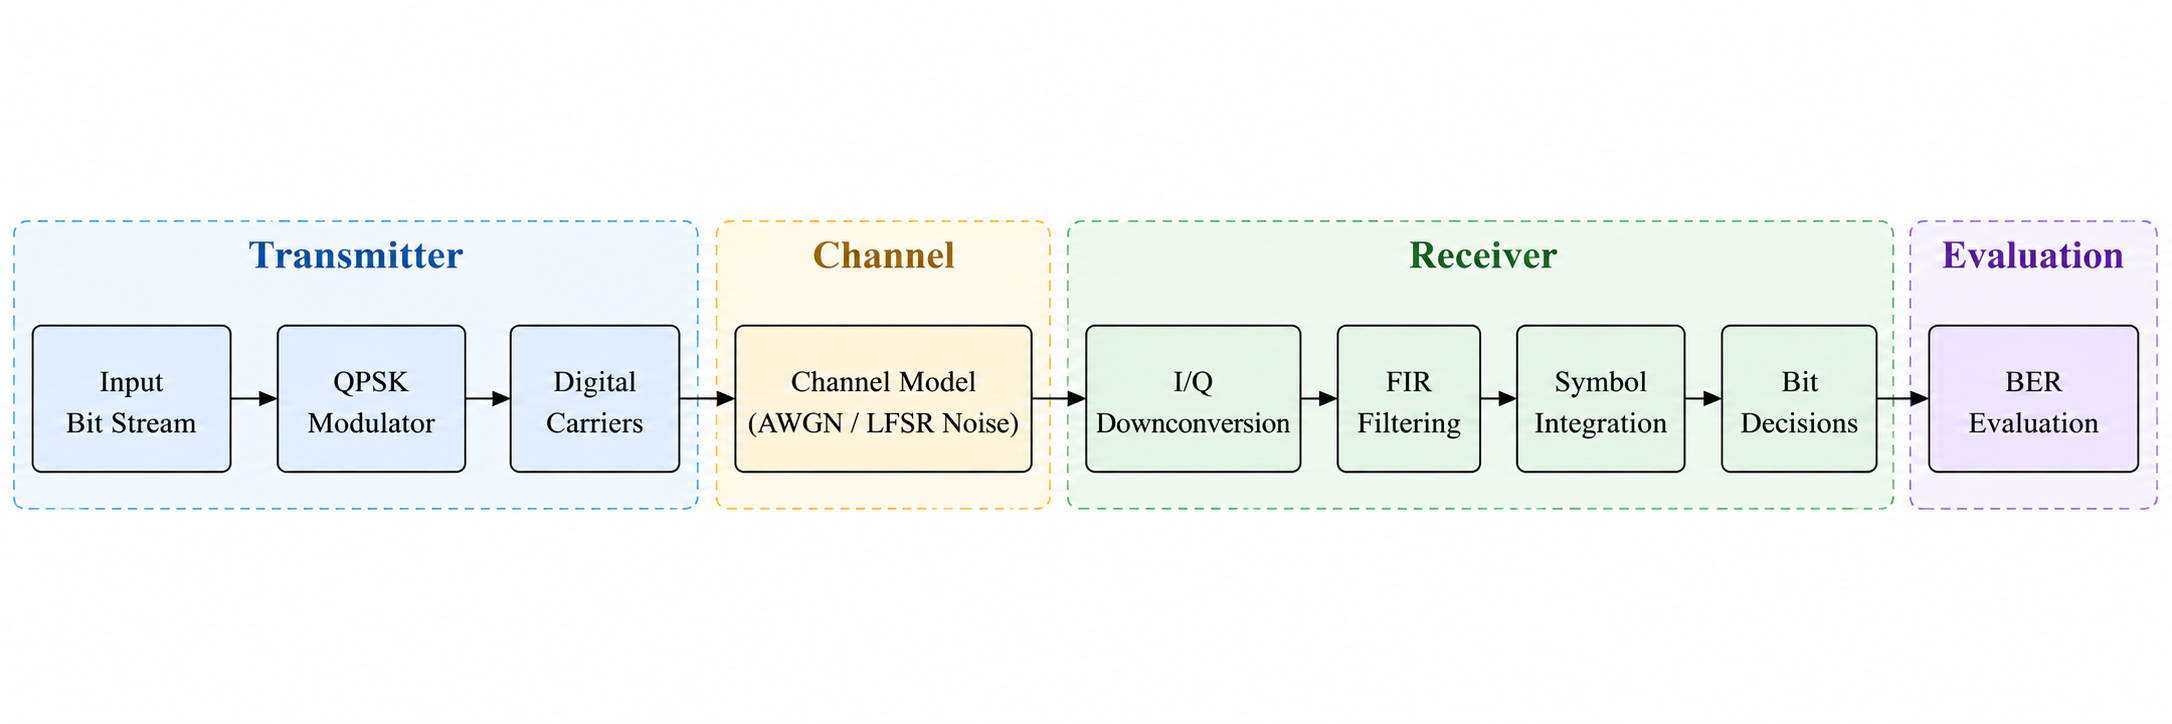
\includegraphics[width=\linewidth]{system_overview.png}
\caption{Block diagram of the QPSK chain as modelled in Python. The UART
constellation output is planned for the hardware stage and is not shown.}
\label{fig:blocks}
\end{figure}

\subsection{Model Parameters}

Table~\ref{tab:params} lists the settings used in the version of the code
reported here (\texttt{params.py} and \texttt{rx\_frontend.py}). If any of
these settings change later, every number in this report has to be rerun.

\begin{table}[t]
\centering\small
\caption{Parameters of the Python golden model.}
\label{tab:params}
\begin{tabular}{@{}p{0.52\linewidth}p{0.44\linewidth}@{}}
\toprule
Parameter & Value \\
\midrule
Samples per symbol $N_s$ & 16 \\
Carrier cycles per symbol & 2 ($f_c/f_s = 0.125$) \\
NCO accumulator / LUT address & 16 bit / 8 bit (256 entries) \\
NCO phase increment & 8192 \\
Datapath (LUT, carrier) & 12 bit signed, full scale 2047 \\
TX mixer output & 13 bit signed \\
RX input word & 12 bit signed, full scale $\pm 8.0$ \\
RX mixer output & 12 bit signed (saturating) \\
FIR & 25 taps (order 24), Hamming-windowed sinc \\
FIR cutoff ($-6$\,dB) & 0.125 cycles/sample \\
FIR coefficients & 12 bit, Q1.11, DC gain exactly 1 \\
FIR group delay & 12 samples \\
Integrate-and-dump accumulator & 16 bit signed \\
\bottomrule
\end{tabular}
\end{table}

\subsection{Bit Source and Mapper}

Two bit sources are used. BER sweeps use NumPy random bits, so the statistics
are not tied to a short repeating pattern. The hardware-oriented source is a
7-bit Fibonacci LFSR (PRBS-7, seed \texttt{0x7F}, feedback $=$ bit~0 $\oplus$
bit~6, shift right), whose period is $2^7-1=127$ bits; the Python model
reproduces the intended Verilog update bit for bit, so the same sequence can
be generated in RTL.

Bit pairs $(b_0,b_1)$ are mapped to symbols by
\begin{equation}
I = 1-2b_0, \qquad Q = 1-2b_1 ,
\end{equation}
so a 0 bit becomes $+1$ and a 1 bit becomes $-1$ on each branch. Writing the
pair as $(I,Q)$, this gives $00\!\to\!(+1,+1)$, $01\!\to\!(+1,-1)$,
$11\!\to\!(-1,-1)$ and $10\!\to\!(-1,+1)$. The four points sit at
$45^\circ$, $315^\circ$, $225^\circ$ and $135^\circ$. Going around the
circle, neighbouring points differ in only one bit (Gray coding). The most
likely mistake is landing in a neighbouring region, and with this mapping
that costs one bit error instead of two.

\subsection{Numerically Controlled Oscillator}

The carrier is produced by a phase accumulator and a sine/cosine lookup table
(LUT). At every sample the 16-bit accumulator adds the increment
\begin{equation}
\Delta\phi = \operatorname{round}\!\left(\frac{f_c}{f_s}\,2^{16}\right)=8192,
\end{equation}
and its upper 8 bits address a 256-entry LUT holding
$\operatorname{round}(2047\cos\theta)$ and $\operatorname{round}(2047\sin\theta)$
as 12-bit two's-complement integers. Because $\Delta\phi$ is a multiple of
$2^{16-8}=256$, every visited phase lands exactly on a LUT entry, so phase
truncation introduces no error for this carrier. The NCO then visits only 8 of
the 256 LUT points (multiples of $45^\circ$), with values
$\{\pm2047,\pm1447,0\}$, and returns to phase zero after every symbol
(two full cycles in 16 samples). The fixed-point transmitter exploits this by
tiling a single symbol of NCO output.

\subsection{QPSK Modulator}

The transmitted samples are
\begin{equation}
s[n] = I[n]\cos(\omega_c n) - Q[n]\sin(\omega_c n),
\end{equation}
with each $I,Q$ value held for $N_s=16$ samples. The minus sign on the
$Q$ branch is a fixed convention shared by transmitter and receiver; changing
it in only one place inverts every $Q$ decision. In the integer model, with
$I,Q\in\{\pm1\}$ the product is exact, and the worst case
$2047\sqrt2\approx 2895$ exceeds the 12-bit range, so the mixer output is
13 bits wide. The model raises an exception instead of wrapping if a value
would not fit.

\subsection{AWGN Channel}

The received samples are $r[n]=s[n]+w[n]$ with white noise $w[n]$ of
variance $\sigma^2$. For the unit-amplitude carrier the mean signal power is
$P=1$, so the symbol energy is $E_s=PN_s$ and, since QPSK carries two bits
per symbol, $E_b=E_s/2$. With $\sigma^2=N_0/2$ per real sample,
\begin{equation}
\sigma^2=\frac{P\,N_s}{4\,(E_b/N_0)} ,
\end{equation}
where $E_b/N_0$ is a linear ratio and $P$ is measured from the signal, so the
same function serves the float and the rescaled integer signal.

Two noise sources are implemented. The reference source is NumPy's standard
normal generator. The hardware-style source is built from a 16-bit LFSR
(feedback taps at bits 0, 2, 3 and 5, period $2^{16}-1=65535$): eight
successive bits form one byte, and six byte streams from different seeds are
summed and normalised to zero mean and unit variance, which approximates a
Gaussian distribution by the central limit theorem. Over $10^5$ samples this
gave a measured mean of $-0.002$ and variance of $1.001$. It is an
approximation rather than true Gaussian noise: the stream repeats every 65535
samples (about 4096 symbols), the six streams are different phases of the same
sequence, and the sum of six bytes has bounded support, so the noise is
truncated at about $\pm4.2\sigma$. The LFSR source is therefore used only for
short runs; all BER sweeps use the NumPy source.

\subsection{Receiver Front End}

The received signal is multiplied by the local references,
\begin{equation}
x_I[n]=r[n]\cos(\omega_c n), \qquad x_Q[n]=-r[n]\sin(\omega_c n),
\end{equation}
which yields $\pm I/2$ and $\pm Q/2$ at baseband plus a component at
$2f_c$. A 25-tap linear-phase low-pass FIR (Hamming-windowed sinc, cutoff
$0.125$ cycles/sample) is applied to each branch. Measured on the
floating-point design, the passband
($f\le 1/16$) stays within $0.1$\,dB of unity and the stopband ($f\ge 3/16$,
where the $2f_c$ product lies) is more than $40$\,dB down. The filter is
causal, so its output is delayed by $D=12$ samples. The model supports either
a causal output, where symbol $k$ starts at sample $16k+D$ and the decision
window is offset by $D$, or an aligned output with zero offset. The two are
verified to give identical decision values (Section~\ref{sec:verif}).

The fixed-point version follows the intended RTL arithmetic. The received
sample is quantised to a 12-bit word with full scale $\pm8.0$ (the TX
amplitude 1.0 corresponds to 256 codes; at $E_b/N_0=0$\,dB $\sigma=2$, so the
range covers $\pm4\sigma$). The mixer computes
$(r_{\mathrm{int}}\,c+2^{10})\gg 11$ with saturation to 12 bits, and the FIR
computes an exact wide sum of products followed by $(\mathrm{acc}+2^{10})\gg 11$
and saturation, where the 12-bit coefficients are in Q1.11 and rounded so that
$\sum h=2048$ (unity DC gain).

\subsection{Integrate-and-Dump and Decision}

Each symbol is recovered by summing 16 consecutive filter outputs,
\begin{align}
\hat I_k&=\sum_{m=0}^{15} y_I[16k+m],\\
\hat Q_k&=\sum_{m=0}^{15} y_Q[16k+m],
\end{align}
which is the matched filter for a rectangular pulse. Because the $2f_c$
product completes exactly four cycles in 16 samples, the sum removes it
completely even without the FIR. For a noiseless symbol, $\hat I_k=\pm8$
(baseband level $\pm0.5\times16$). The bit decision is
\begin{equation}
\hat b_0=\begin{cases}0,&\hat I_k\ge 0\\1,&\hat I_k<0\end{cases}
\end{equation}
and the same rule is used for $\hat b_1$ with $\hat Q_k$. A value of exactly
zero is decided as bit 0. In the integer model the
accumulator needs $12+\log_2 16=16$ signed bits. When counting errors the
first and last symbols are skipped, because they see filter start-up and
cut-off.

\subsection{BER Analysis}

For ideal coherent QPSK in AWGN the reference curve is
\begin{equation}
P_b=Q\!\left(\sqrt{2E_b/N_0}\right).
\end{equation}
For the actual receiver (mixer, FIR, 16-sample integration) the model also
computes an exact prediction without random simulation. The decision value of
a symbol depends only on that symbol and its neighbours, so the noiseless
chain is evaluated for all $4^3=64$ three-symbol neighbourhoods to obtain the
signal margin $d$. The decision-noise variance follows in closed form from the
combined kernel $g=\mathrm{box}_{16}\ast h$, and the BER is the average of
$Q(d/\sigma_d)$ over the neighbourhoods. Simulated results are compared with
the matching prediction using a $z$-score
\begin{equation}
z=\frac{N_{\mathrm{err}}-N p}{\sqrt{Np(1-p)}},
\end{equation}
and the number of simulated bits
at each $E_b/N_0$ is chosen so that about 100 errors are expected (capped at
$1.5\times10^6$ bits).

\subsection{Verification Procedure}
\label{sec:verif}

We check the model in stages, so that each check looks for one kind of
mistake. The noiseless test comes first. If the chain cannot recover the bits
with no noise, something is wrong with the mapping, the signs or the bit
order, and no BER number should be trusted. Next we check the filter delay:
the causal FIR output, read with a 12-sample offset, must give the same
decision values as the aligned output. Then we run BER sweeps and compare
them with the QPSK formula and with the exact prediction for our FIR
receiver. After that we run the integer (fixed-point) chain on the same bits
and noise as the floating-point chain and compare the two. Last, we run a
short test with the LFSR noise source and export the golden vectors. All of
these checks are \texttt{assert} statements in the scripts, so a failed check
stops the run. Table~\ref{tab:checks} summarises them and their outcome.

\begin{table}[t]
\centering
\small
\begin{tabular}{@{}p{0.31\linewidth}p{0.65\linewidth}@{}}
\toprule
Check & Purpose and outcome \\
\midrule
Noiseless end-to-end test & Zero bit errors for the tested floating-point and fixed-point receiver variants. \\
FIR delay alignment & The causal FIR decisions agree with the aligned FIR decisions for 499 of 500 compared symbols when the 12-sample delay is accounted for. \\
BER sweep & The no-FIR BER agrees with theoretical coherent-QPSK BER; the FIR BER agrees with the prediction for the implemented FIR receiver within the observed statistical variation. \\
Fixed-point comparison & At 4 dB, the fixed-point and floating-point BER values are 0.01436 and 0.01435, respectively, using the same bits and noise. \\
LFSR noise test & At 2 dB, the LFSR-based run gives BER 0.0391 compared with a model prediction of 0.0415. \\
Golden-vector export & The exported files are read back and checked against the arrays written by the Python script. \\
\bottomrule
\end{tabular}
\caption{Summary of the current Python-model verification checks. These checks do not represent RTL or FPGA verification.}
\label{tab:checks}
\end{table}

\subsection{Golden Vectors for RTL}
The fixed-point script exports six hexadecimal files for later verification of the integrate-and-dump and decision stages. The files contain transmitted bits, filtered I and Q samples, the I and Q accumulator values, and received bits. The export covers 127 symbols, uses a 12-sample timing offset and 16-bit signed accumulators, and passes through the LFSR-based noise channel at 6 dB. The comparison contains 250 bits and produces zero errors for this test. The files are read back and checked against the arrays that were written. They are reference inputs and outputs for a future RTL testbench; their generation does not show that any RTL has passed.

\subsection{Scope and Assumptions}
\label{sec:scope}

The receiver assumes known carrier phase and symbol timing, with the local
carrier locked to the transmitter. There is no carrier or timing recovery in
the current model; the Costas loop, Gardner timing recovery and a coded
comparison remain optional extensions. All results in this report come from
the Python model; nothing here has been run in RTL or on the FPGA.

% =====================================================================
\section{Results Replicated from the Literature}

\subsection{Theoretical BER of coherent QPSK}
A standard reference result for coherent QPSK in an additive white Gaussian noise (AWGN) channel is the theoretical bit-error rate (BER)~\cite{proakis}:
\begin{equation}
 P_b=Q\!\left(\sqrt{\frac{2E_b}{N_0}}\right),
 \label{eq:qpsk_ber_theory}
\end{equation}
where $E_b/N_0$ is the bit-energy-to-noise-density ratio and $Q(\cdot)$ is the Gaussian tail probability. This result is used as the analytical reference for the present simulations. With rectangular symbol pulses and ideal carrier and timing alignment, the receiver without the FIR uses mixing followed by a 16-sample integrate-and-dump operation. Its simulated BER is expected to follow Equation~\ref{eq:qpsk_ber_theory}.

Table~\ref{tab:ber} shows that the no-FIR results are close to the theoretical values at all five tested points. The normalized differences are within $|z|\leq 1.5$ for this run, consistent with the statistical variation expected from a finite number of transmitted bits. The comparison also provides a check of the implemented noise scaling. Figure~\ref{fig:fixed_ber} shows the same comparison on a log scale, with the simulated points sitting on the curves. The FPGA papers we reviewed focus mainly on architecture and device-specific implementation results, so this report does not claim to reproduce their particular FPGA resource counts or hardware measurements.

\subsection{DDS frequency relation}
Song and Yao~\cite{song2010qpsk} give the output frequency of a DDS/NCO as
$f_{\mathrm{out}}=Kf_{\mathrm{clk}}/2^M$
(Eq.~\ref{eq:dds_frequency}). We checked our NCO against it. With $M=16$ and
$K=8192$ the formula gives $f_{\mathrm{out}}=f_{\mathrm{clk}}/8$, that is
$f_c/f_s=0.125$, or two carrier cycles in each 16-sample symbol, as intended.
In our simulated NCO the output repeats every 8 samples. The cosine goes
$2047,\,1447,\,0,\,-1447,\,-2047,\,-1447,\,0,\,1447$, and the sine is the
same list delayed by two samples. These are the stored 12-bit values of
cosine and sine at multiples of $45^\circ$. The only difference from an ideal
sinusoid is rounding to whole numbers, at most half a code (for example,
$2047\cos 45^\circ=1447.4$ is stored as $1447$), which is under
$0.03\,\%$ of full scale. We built the NCO with the same structure as the
paper, so this agreement is expected. It confirms that our implementation is
correct; it is not a new result.

\subsection{QPSK signal and constellation}
The NPTEL notes~\cite{nptel_qpsk} write the QPSK signal as
$s_i(t)=\sqrt{2E/T}\cos\!\big(2\pi f_ct+(2i-1)\pi/4\big)$ for $i=1,\dots,4$,
so the four symbols sit at $45^\circ$, $135^\circ$, $225^\circ$ and
$315^\circ$, and the signal behaves like two BPSK signals on orthogonal
carriers. Our transmitted signal can be rewritten as
$I\cos\omega_cn-Q\sin\omega_cn=\sqrt2\cos(\omega_cn+\phi)$ with
$\phi=\operatorname{atan2}(Q,I)$. For our mapping this gives exactly the same four
phases: $(+1,+1)$ at $45^\circ$, $(-1,+1)$ at $135^\circ$, $(-1,-1)$ at
$225^\circ$ and $(+1,-1)$ at $315^\circ$. The receiver constellations in
Fig.~\ref{fig:const} show four clusters around $(\pm1,\pm1)$, as expected.
The notes also describe a correlation receiver that multiplies by the two
carriers and integrates over a symbol. Our mixer followed by integrate-and-dump
is the sampled version of that receiver.

\subsection{What we have not replicated}
The FPGA papers we reviewed report hardware results (clock speeds, device
resource use and oscilloscope measurements). Our design has not been
synthesised or run on a board yet, so we do not claim to reproduce any of
those numbers.

% =====================================================================
\section{Preliminary Results}

\subsection{Noiseless Correctness}
With noise disabled, the floating-point chain gives zero bit errors in the tested receiver variants: no FIR, 0/3996 bits; aligned FIR, 0/3996 bits; and causal FIR, 0/3994 bits. For the no-FIR case, the decision values are exactly $\pm 8=\pm N_s/2$, where $N_s=16$ samples per symbol. The fixed-point chain also gives zero errors for all three variants. In the noiseless fixed-point test, the maximum accumulator magnitudes are 2048 without the FIR and 2132 for the tested FIR path.

When the FIR delay is handled using an offset of $D=12$ samples, the causal and aligned FIR decisions match for 499 of the 500 compared symbols. Using no offset does not give the same result. This confirms that the FIR delay must be accounted for when locating symbol-decision intervals.

\subsection{BER versus $E_b/N_0$}
Table~\ref{tab:ber} shows the integer-chain BER with and without the FIR, alongside theoretical coherent-QPSK BER and the prediction for the implemented FIR receiver. Each point uses approximately 100,000 bits, except the 8 dB point, which uses 599,976 bits. BER decreases as $E_b/N_0$ increases. Each measured value lies within $|z|\leq 1.9$ of its corresponding prediction for this run.

The FIR does not improve BER in the present receiver arrangement. In the floating-point model, its estimated penalty rises from about 0.215 dB at 0 dB to about 0.337 dB at 8 dB. One possible explanation is that the FIR spreads symbol transitions, while the 16-sample integrate-and-dump operation already suppresses the doubled-carrier component under the assumed alignment. The filter is retained because it is part of the planned receiver architecture, not because it improves the current simulated BER. At 8 dB, the simulated BER values are below their predictions; the number of errors is relatively small, so a longer run would provide a more precise comparison.

\begin{table*}[t]
\centering
\small
\begin{tabular}{@{}rcccc@{}}
\toprule
$E_b/N_0$ (dB) & No FIR & Theory & FIR & FIR prediction \\
\midrule
0 & $7.831\times10^{-2}$ & $7.865\times10^{-2}$ & $8.400\times10^{-2}$ & $8.385\times10^{-2}$ \\
2 & $3.745\times10^{-2}$ & $3.751\times10^{-2}$ & $4.120\times10^{-2}$ & $4.145\times10^{-2}$ \\
4 & $1.301\times10^{-2}$ & $1.250\times10^{-2}$ & $1.500\times10^{-2}$ & $1.472\times10^{-2}$ \\
6 & $2.320\times10^{-3}$ & $2.388\times10^{-3}$ & $3.070\times10^{-3}$ & $3.159\times10^{-3}$ \\
8 & $1.650\times10^{-4}$ & $1.909\times10^{-4}$ & $2.717\times10^{-4}$ & $3.162\times10^{-4}$ \\
\bottomrule
\end{tabular}
\caption{Simulated BER of the integer chain compared with theoretical QPSK BER and the prediction for the implemented FIR receiver.}
\label{tab:ber}
\end{table*}

\begin{figure}[t]
\centering
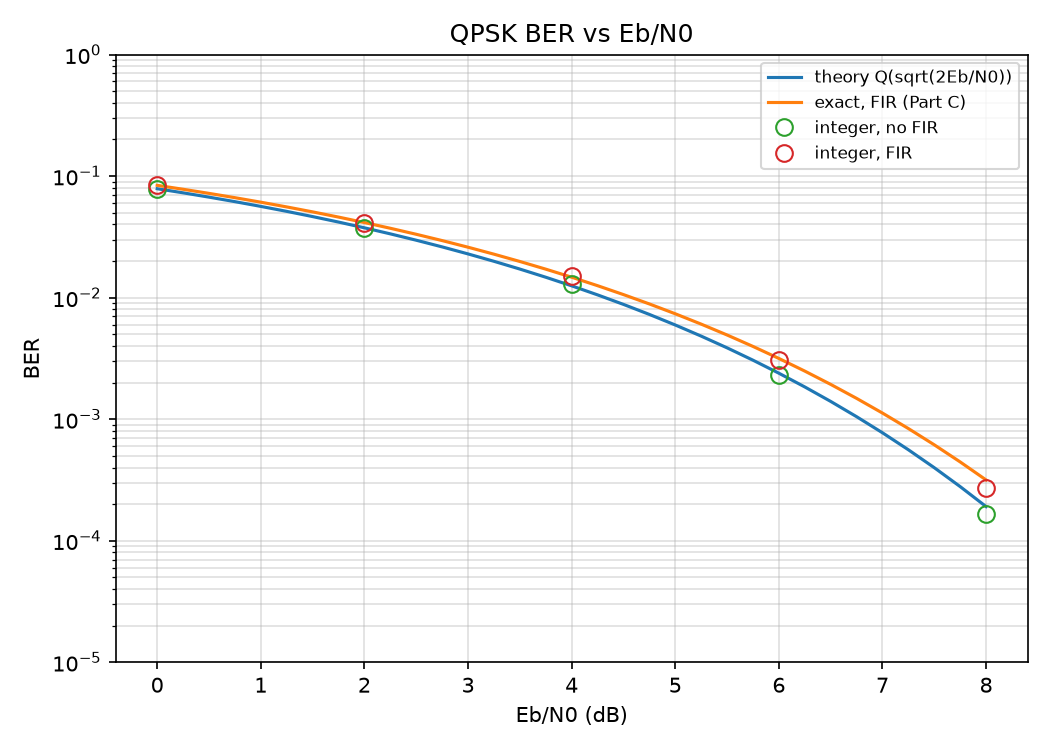
\includegraphics[width=\linewidth]{fixed_ber_curve.png}
\caption{BER versus $E_b/N_0$ for the fixed-point (integer) chain, with and without the FIR, compared with the theoretical QPSK curve and the exact prediction for the FIR receiver.}
\label{fig:fixed_ber}
\end{figure}

\subsection{Constellation Plots}
Figure~\ref{fig:const} shows the receiver decision values at 0, 6, and 12 dB. The four clusters become more compact as $E_b/N_0$ increases. At 0 dB, the clusters spread across the decision boundaries, which is consistent with the higher BER. The values in the plot are scaled for display; the raw accumulator outputs are not limited to $\pm1$.

\begin{figure*}[t]
\centering
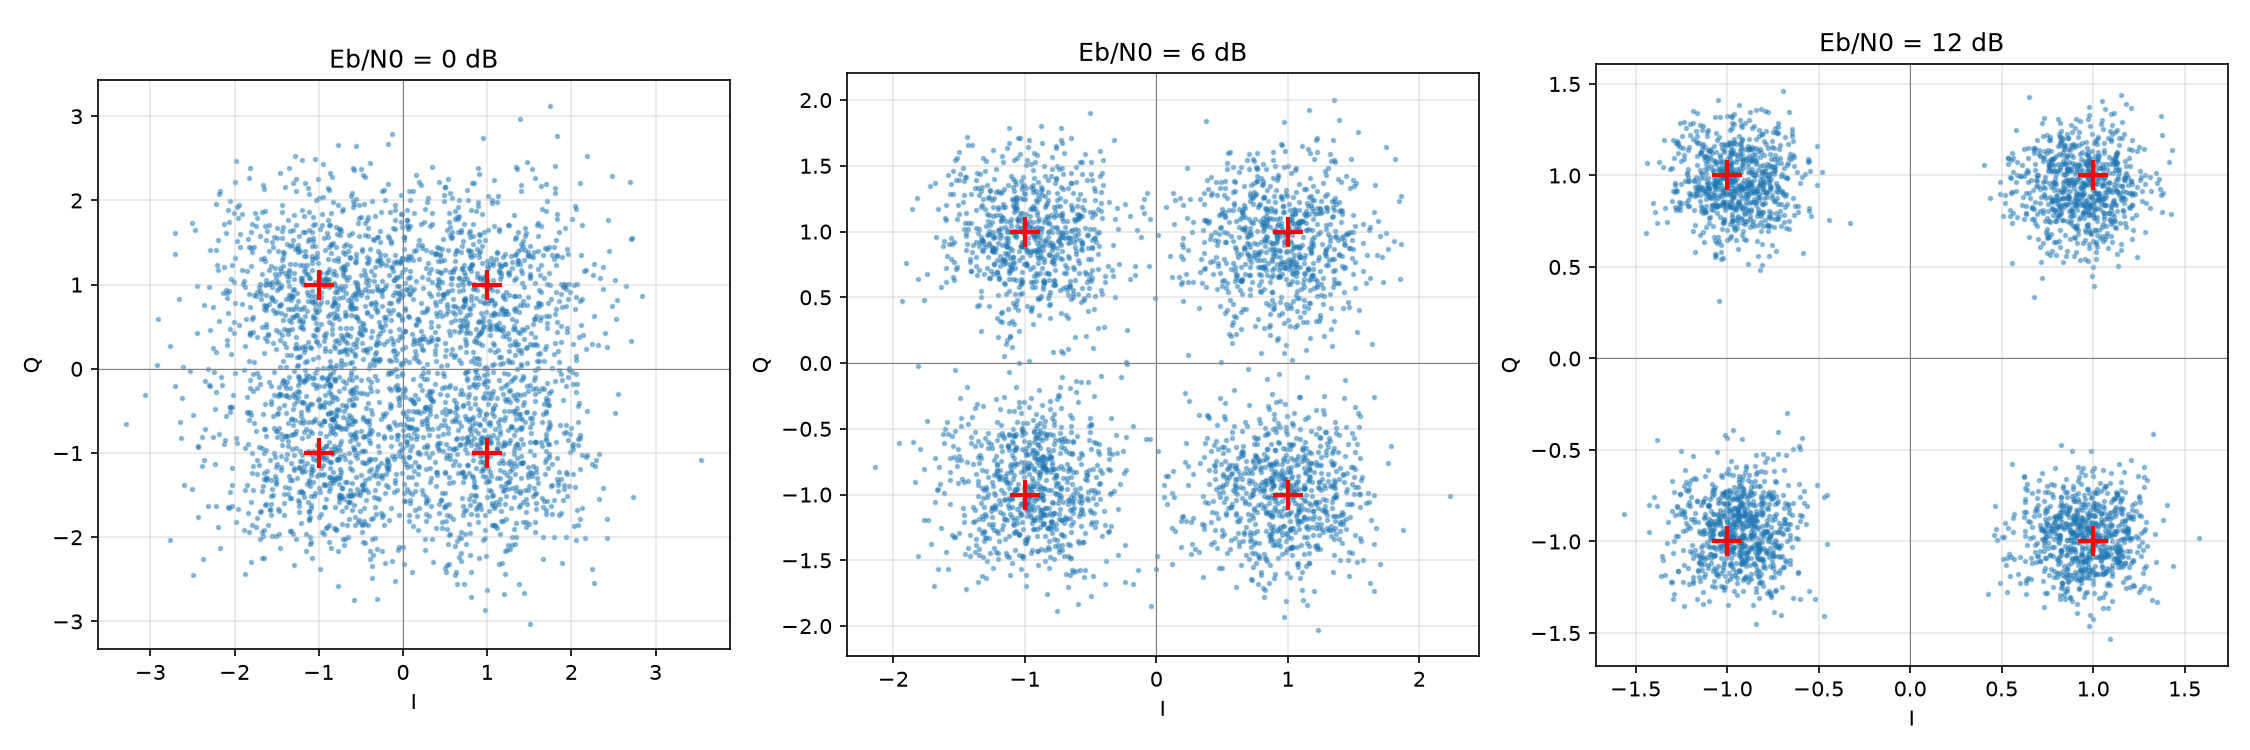
\includegraphics[width=0.9\textwidth]{fixed_constellations.png}
\caption{Receiver constellations of the fixed-point chain at 0, 6, and 12 dB. The red crosses mark the ideal points $(\pm1,\pm1)$.}
\label{fig:const}
\end{figure*}

\subsection{Fixed-Point versus Floating-Point Model}
At 4 dB, using the same transmitted bits and noise, the fixed-point chain gives BER 0.01436 and the floating-point chain gives BER 0.01435. The RMS difference between their decision values is 0.0009 on a normalized noiseless level of 1. The input clipping fraction is zero, and the maximum accumulator magnitude is 6066, compared with a 16-bit signed limit of 32767. Therefore, no accumulator overflow occurred in this test. Since this comparison was performed at one noise level, it should not be taken as proof that the two implementations agree equally well at every $E_b/N_0$.

\subsection{LFSR-Based Noise Test}
Using the hardware-oriented LFSR noise source, a run of 4000 symbols at 2 dB gives BER 0.0391 compared with a model prediction of 0.0415. The measured value is approximately one standard deviation below the prediction and is consistent with the expected variation for this run. The LFSR sequence is deterministic and periodic, so it is treated as an approximation for hardware-oriented testing. The BER sweeps in Table~\ref{tab:ber} use NumPy-generated Gaussian noise instead.

% =====================================================================
\section{Discussion, Limitations and Plan}

\paragraph{What the results show.}
The Python tests support the consistency of the transmitter/receiver sign and bit-order conventions implemented in the model, the handling of FIR delay, and the AWGN scaling used in the BER sweep. At the tested word lengths and signal scale, the fixed-point results are close to the floating-point reference. The 12-bit datapath, 13-bit transmitter mixer output, and 16-bit accumulator provide a starting point for RTL design, subject to verification of widths and signed arithmetic in the hardware implementation.

\paragraph{Limitations.}
The current receiver assumes known carrier phase and symbol timing, so carrier-frequency/phase offsets and timing errors are not handled. The LFSR-based noise source is a periodic approximation and is not used for the main BER sweep. The fixed-point versus floating-point comparison has been reported at one $E_b/N_0$ point only. Finally, no RTL simulation or FPGA test has been completed, so resource utilization, timing closure, and real-time board behaviour remain unknown.

\paragraph{Plan for the final stage.}
The next stage is to implement and simulate the NCO, mapper, transmitter mixer, receiver mixer, FIR filter, integrate-and-dump logic, and decision logic in Verilog. The RTL outputs will be compared with the exported golden vectors. After block-level verification, the design will be integrated on the RealDigital Boolean Board with the Spartan-7 XC7S50, and the LUT, flip-flop, DSP, and memory use will be recorded. If supported by the remaining time, a UART-based constellation output and hardware BER measurements will be added and compared with the Python reference model. Optional extensions include carrier recovery using a Costas loop, timing recovery using a Gardner detector, and a comparison of coded and uncoded BER.

% =====================================================================
\section{Conclusion}
This report presented the mid-term state of a QPSK modem planned for the
Boolean Board. So far the transmitter, noisy channel, receiver and BER
measurement exist as floating-point and fixed-point Python models. The chain
recovers every bit when there is no noise. With noise, the simulated BER
follows the coherent-QPSK formula for the receiver without the FIR, and
follows the exact prediction for the receiver with it, within the normal
statistical spread ($|z|\le 1.5$ and $|z|\le 1.9$ over the five tested
points). The FIR costs about 0.2 to 0.34~dB of $E_b/N_0$, so it does not help
BER in the current setup. At 4~dB the fixed-point model gives a BER of
0.01436 against 0.01435 for floating point, with no input clipping and an
accumulator peak of 6066 out of a 16-bit limit of 32767. The LFSR-based noise
test gave 0.0391 against a predicted 0.0415, and golden vectors for 127
symbols were exported for later testing.

These are Python results only. No Verilog has been simulated and nothing has
been run on the FPGA yet. The next step is to write and simulate the RTL
blocks, compare them with the golden vectors, and then bring the design up on
the Boolean Board.

% =====================================================================
% \section{Work Distribution and AI Use}

% \subsection{Work Distribution}
% The Python model is split into four parts, each owned by one member.

% \begin{table}[t]
% \centering
% \small
% \begin{tabular}{@{}p{0.26\linewidth}p{0.64\linewidth}@{}}
% \toprule
% Team member & Contribution \\
% \midrule
% Parth & Part A: PRBS-7 bit source, QPSK mapper, NCO (floating-point and fixed-point), transmitter mixer, LUT hex export. \\
% Nishid & Part B: AWGN channel (NumPy and LFSR noise), fixed-point helpers, theoretical BER. \\
% Aditya & Part C: receiver mixer, FIR design and quantisation, exact BER prediction for the FIR receiver. \\
% Darsh & Part D: integrate-and-dump, bit decisions, BER counter and sweep, end-to-end runner, plots, golden vectors. \\
% All members & Literature review and report writing: \fillme{FILL: who wrote which section}. \\
% \bottomrule
% \end{tabular}
% \caption{Distribution of project work among team members.}
% \label{tab:work_distribution}
% \end{table}

% \subsection{Use of AI Tools}
% We used AI tools in this project, as the course allows. The file headers of
% \texttt{rx\_frontend.py}, \texttt{rx\_backend\_eval.py} and \texttt{main.py}
% state that their first drafts were written with Claude (Sonnet 5.5,
% Anthropic). For Parts A and B: \fillme{FILL: say exactly what AI was or was not used
% for}. We also used Claude to help plan the report, draft and tidy the text of
% several sections, and explain technical ideas. All numbers in the report come
% from our own scripts and their output, and we checked them against the logs
% and plots before submission. Each member can explain the parts they own,
% including the equations, the fixed-point choices, the noise generation and the
% tests.

% =====================================================================
{\small
\bibliographystyle{ieee_fullname}
\bibliography{references}
}

\end{document}
